\documentclass[preprint,12pt,aps,pra,showkeys,amsmath,amssymb,superscriptaddress,floatfix]{revtex4-2}
\usepackage[T1]{fontenc}
\usepackage[utf8]{inputenc}
\usepackage{amsmath,amssymb,amsthm,mathtools,mathrsfs}
\usepackage{microtype,booktabs,enumitem}
\usepackage{xcolor,tikz,etoolbox}
\usepackage[skins,breakable]{tcolorbox}
\usepackage{needspace}
% Keep diagram geometry independent of REVTeX preprint body spacing.
\AtBeginEnvironment{tikzpicture}{\linespread{1}\selectfont}
\usetikzlibrary{arrows.meta,positioning,calc,fit,decorations.pathreplacing}
\usepackage{graphicx}
\usepackage{hyperref}

\definecolor{MMBlue}{RGB}{0,82,155}
\definecolor{MMOrange}{RGB}{200,80,0}
\tikzset{
 mmnode/.style={draw=MMBlue,rounded corners=2pt,fill=MMBlue!4,align=left,execute at begin node={\raggedright},text width=5cm,font=\fontsize{10}{12}\selectfont,inner sep=6pt},
 mmimport/.style={mmnode,draw=black!65,fill=black!4},
 mmcandidate/.style={mmnode,draw=MMOrange,dashed,fill=MMOrange!5},
 mmrejected/.style={mmnode,draw=black,densely dotted,fill=black!8},
 mmproof/.style={->,thick,MMBlue},
 mmflow/.style={->,semithick,black!70},
 mmrepair/.style={->,dashed,thick,MMOrange},
 mmcandidatearrow/.style={->,dashed,semithick,MMOrange},
 mmnote/.style={font=\scriptsize,fill=white,inner sep=2pt,align=center}}

\usepackage[section]{placeins}
\setlength{\emergencystretch}{3em}
\setlist{itemsep=3pt,topsep=4pt}
\newtheorem{theorem}{Theorem}[section]
\newtheorem{proposition}[theorem]{Proposition}
\newtheorem{lemma}[theorem]{Lemma}
\newtheorem{corollary}[theorem]{Corollary}
\theoremstyle{definition}
\newtheorem{definition}[theorem]{Definition}
\newtheorem{example}[theorem]{Example}
\theoremstyle{remark}
\newtheorem{remark}[theorem]{Remark}
% Avoid isolated statement headings and single-line paragraph fragments.
\BeforeBeginEnvironment{theorem}{\Needspace{6\baselineskip}}
\BeforeBeginEnvironment{definition}{\Needspace{5\baselineskip}}
\BeforeBeginEnvironment{proposition}{\Needspace{5\baselineskip}}
\BeforeBeginEnvironment{lemma}{\Needspace{5\baselineskip}}
\BeforeBeginEnvironment{corollary}{\Needspace{5\baselineskip}}
\clubpenalty=5000
\widowpenalty=5000
\newcommand{\R}{\mathbb R}\newcommand{\Z}{\mathbb Z}\newcommand{\N}{\mathbb N}
\newcommand{\Pa}{\operatorname{Pa}}\newcommand{\Desc}{\operatorname{Desc}}
\newcommand{\cl}{\operatorname{cl}}\newcommand{\cost}{\operatorname{cost}}
\newcommand{\status}{\operatorname{status}}
% Faculty cards: a visual rail groups the five faculties within one agent.
% The rail has no arrowhead and does not represent a proof dependency.
\newcommand{\mmfacultybadge}[1]{%
 \node[circle,draw=MMBlue,line width=1pt,fill=white,
 minimum size=7mm,inner sep=0pt,font=\sffamily\small\bfseries,text=MMBlue]
 at ([xshift=15pt,yshift=-15pt]frame.north west) {#1};}
\newcommand{\mmfacultyrail}{%
 \draw[MMBlue!80,line width=1pt]
 ([xshift=15pt,yshift=2pt]frame.north west)--
 ([xshift=15pt,yshift=-2pt]frame.south west);}
\newtcolorbox{mmfacultybox}[2]{enhanced,breakable,
 colback=MMBlue!4,colframe=MMBlue!4,boxrule=0pt,arc=3pt,
 left=39pt,right=9pt,top=7pt,bottom=7pt,
 before skip=2pt,after skip=2pt,
 fontupper=\normalsize\linespread{1.15}\selectfont,
 overlay unbroken={\mmfacultyrail\mmfacultybadge{#1}},
 overlay first={\mmfacultyrail\mmfacultybadge{#1}},
 overlay middle={\mmfacultyrail},overlay last={\mmfacultyrail}}
\newcommand{\mmfaculty}[3]{%
 \begin{mmfacultybox}{#1}{#2}
 {\sffamily\bfseries\color{MMBlue}#2}\par\smallskip #3
 \end{mmfacultybox}}
\newcommand{\agent}[9]{%
 \Needspace{8\baselineskip}
 \subsubsection{#1}
 \noindent\textbf{Object.} #2\par
 \noindent\textbf{Role.} #3\par\smallskip
 \mmfaculty{E}{Ego}{#4}
 \mmfaculty{M}{Memory}{#5}
 \mmfaculty{I}{Intellect}{#6}
 \mmfaculty{S}{Sense}{#7}
 \mmfaculty{A}{Action}{#8}
 \smallskip\noindent #9\par}

\usepackage{longtable,array}
\providecommand{\tightlist}{\setlength{\itemsep}{2pt}\setlength{\parskip}{0pt}}
% Keep short report abstracts with their title instead of REVTeX's optional preprint break.
\makeatletter
\def\frontmatter@abstract@produce{\par\addvspace{\frontmatter@preabstractspace}%
\begingroup\prep@absbox\unvbox\absbox\post@absbox\endgroup
\addvspace{\frontmatter@postabstractspace}}
\makeatother
\newcommand{\field}[2]{\par\smallskip\noindent\textbf{#1.} #2\par}
\newcommand{\reportcaption}[1]{\par\smallskip{\small\noindent #1\par}}


\hypersetup{colorlinks=true,linkcolor=MMBlue,urlcolor=MMBlue,pdftitle={Chinese Remainder Theorem},pdfauthor={Dibakar Sigdel}}

\begin{document}

\title{Chinese Remainder Theorem\\[4pt]\large An End-to-End Meta-Math Walkthrough}

\author{Dibakar Sigdel}

\affiliation{Mindverse Computing LLC, Lynnwood, WA 98087, USA}

\date{October 2026}

\begin{abstract}

Build a selector for each congruence, combine the selectors, and prove
that two solutions differ by the product of the pairwise coprime moduli.
This report presents a complete proof relative to explicit imports, a
dependency graph, versioned node contracts, five-faculty activities,
exact examples, and an illustrative repair. The interactions are
authored explanations, not a transcript of deployed agents or a
proof-assistant certificate.

\end{abstract}

\maketitle

\linespread{1.12}\selectfont

\noindent\textbf{Project NT-03 \quad Report version 1 \quad Number Theory}

\section{Target and import contract}

\begin{theorem}

Let \(k\ge1\), let \(m_1,\ldots,m_k\ge2\) be pairwise coprime integers,
and let \(r_1,\ldots,r_k\in\mathbb Z\). With \(M=\prod_i m_i\), the
system \(x\equiv r_i\pmod{m_i}\) has exactly one solution class modulo
\(M\), and an explicit integer representative can be constructed.

\end{theorem}

\subsection{Foundations and permitted imports}

\begin{enumerate}
\def\labelenumi{\arabic{enumi}.}
\item
  NT-01/N5, v1: if \(\gcd(u,m)=1\) with \(m\ge2\), Bézout constructs
  \(t,s\in\mathbb Z\) such that \(tu+sm=1\).
\item
  NT-02/N1 and N2, v1: every integer greater than \(1\) has a prime
  divisor, and a prime dividing a finite product divides one factor.
  These justify coprimality of complementary and partial products. Empty
  products equal \(1\).
\end{enumerate}

\clearpage\section{Node interaction workflow}

\begin{center}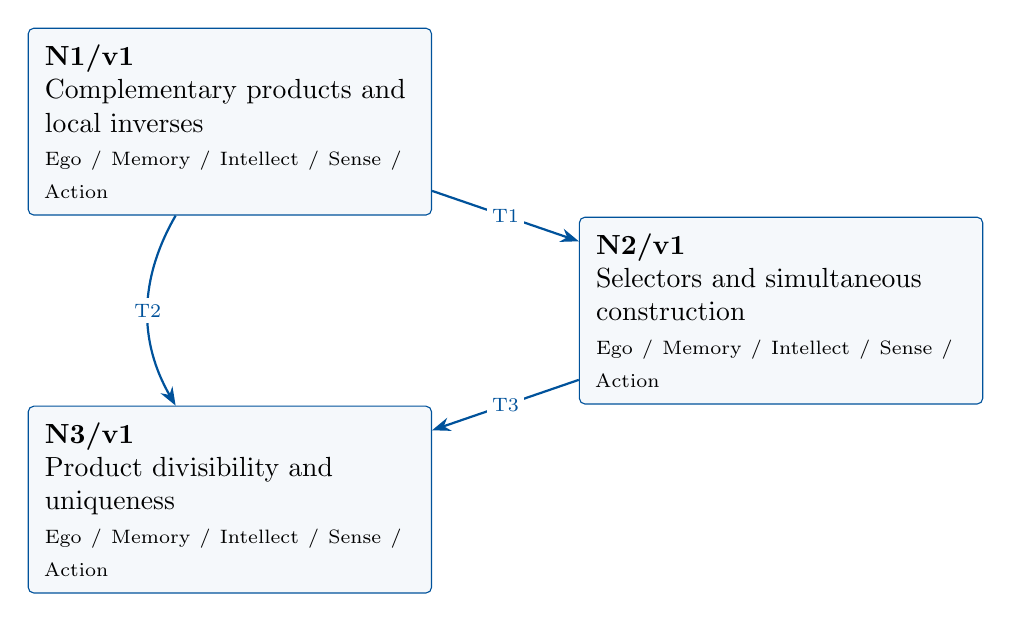
\begin{tikzpicture}[>=Stealth,x=1cm,y=1cm]

\node[mmnode,text width=4.7cm,minimum height=1.35cm] (N1) at (0,0) {\textbf{N1/v1}\\Complementary products and local inverses\\{\scriptsize Ego / Memory / Intellect / Sense / Action}};

\node[mmnode,text width=4.7cm,minimum height=1.35cm] (N2) at (7,-2.4) {\textbf{N2/v1}\\Selectors and simultaneous construction\\{\scriptsize Ego / Memory / Intellect / Sense / Action}};

\node[mmnode,text width=4.7cm,minimum height=1.35cm] (N3) at (0,-4.8) {\textbf{N3/v1}\\Product divisibility and uniqueness\\{\scriptsize Ego / Memory / Intellect / Sense / Action}};

\draw[mmproof] (N1) to node[mmnote,pos=.5] {T1} (N2);

\draw[mmproof,bend right=30] (N1) to node[mmnote,pos=.5] {T2} (N3);

\draw[mmproof] (N2) to node[mmnote,pos=.5] {T3} (N3);

\end{tikzpicture}\end{center}

\reportcaption{Blue arrows are accepted mathematical dependencies, with exact transfers T1--T3 below. Repair messages are described separately; they are not premises of the proof.}

\subsection{Versioned evidence-transfer ledger}

\begingroup\small\linespread{1.05}\selectfont\renewcommand{\field}[2]{\par\noindent\textbf{#1.} #2\par}

\Needspace{5\baselineskip}\smallskip\noindent\textbf{T1: N1/E1 v1 to N2.2–3}

\field{Claim}{For \(M_i=M/m_i\), \(\gcd(M_i,m_i)=1\) and integers \(t_i,s_i\) satisfy
\(t_iM_i+s_im_i=1\). Any product of distinct other moduli is also
coprime to \(m_i\).}

\field{Compatibility}{All selectors use their matching modulus and inverse certificate.}

\field{Evidence}{Node N1 activities below and the continuous proof in Section~\ref{sec:proof}.}

\Needspace{5\baselineskip}\smallskip\noindent\textbf{T2: N1/E1 v1 to N3.2}

\field{Claim}{For \(M_i=M/m_i\), \(\gcd(M_i,m_i)=1\) and integers \(t_i,s_i\) satisfy
\(t_iM_i+s_im_i=1\). Any product of distinct other moduli is also
coprime to \(m_i\).}

\field{Compatibility}{The transferred export includes partial-product coprimality, not just
inverse values.}

\field{Evidence}{Node N1 activities below and the continuous proof in Section~\ref{sec:proof}.}

\Needspace{5\baselineskip}\smallskip\noindent\textbf{T3: N2/E2 v1 to N3.3}

\field{Claim}{\(x=\sum_i r_iM_it_i\) satisfies \(x\equiv r_j\pmod{m_j}\) for every
\(j\).}

\field{Compatibility}{At least one simultaneous solution exists for the fixed residue tuple.}

\field{Evidence}{Node N2 activities below and the continuous proof in Section~\ref{sec:proof}.}

\endgroup

\clearpage\section{Agent roles and five-faculty activities}

\subsection{N1/v1: Complementary products and local inverses}

\field{Object and role}{Construct one certified unit for each modulus and retain the
product-coprimality lemma needed by uniqueness.}

\field{Inputs}{Pairwise coprime \(m_i\ge2\); NT-01 and the declared NT-02 lemmas.}

\mmfaculty{E}{Ego}{Publish each local inverse with its own modulus; retain the coprimality
lemma in the same export.}

\mmfaculty{M}{Memory}{Retain the indexed moduli and prime-divisor/finite-product lemmas.}

\mmfaculty{I}{Intellect}{A shared prime with a complementary product would divide a different
modulus, contradicting pairwise coprimality.}

\mmfaculty{S}{Sense}{The gcd of all moduli being \(1\) is weaker than pairwise coprimality.
For \(k=1\), \(M_1=1\).}

\mmfaculty{A}{Action}{Set \(M=\prod_i m_i\) and \(M_i=M/m_i\). Continue with the numbered
deductions below, retaining the exact export.}

\smallskip\noindent\textbf{Numbered mathematical activities}

\begin{enumerate}[label=N1.\arabic*,leftmargin=3.4em]

\item Set \(M=\prod_i m_i\) and \(M_i=M/m_i\).

\item If a common divisor with \(m_i\) exceeded \(1\), choose a prime divisor
and use Euclid's lemma to contradict pairwise coprimality; the same
argument applies to any partial product.

\item Use Bézout to find \(t_iM_i+s_im_i=1\) for every \(i\).

\end{enumerate}

\field{Export E1/v1}{For \(M_i=M/m_i\), \(\gcd(M_i,m_i)=1\) and integers \(t_i,s_i\) satisfy
\(t_iM_i+s_im_i=1\). Any product of distinct other moduli is also
coprime to \(m_i\).}

\field{Acceptance gate}{Every local inverse and every partial-product coprimality claim refers
to the original indexed moduli.}

\field{Targeted repair}{If pairwise coprimality fails, stop this construction. A generalized CRT
would need a separately stated contract; recheck N2 and N3.}

\clearpage

\subsection{N2/v1: Selectors and simultaneous construction}

\field{Object and role}{Combine independent local certificates into one integer satisfying every
congruence.}

\field{Inputs}{N1/E1 and arbitrary integer residues \(r_i\).}

\mmfaculty{E}{Ego}{Publish existence only after checking each coordinate.}

\mmfaculty{M}{Memory}{Retain inverse certificates with their indices and the divisibility
\(m_j\mid M_i\) for \(i\ne j\).}

\mmfaculty{I}{Intellect}{Each selector \(M_it_i\) is \(1\) at its own modulus and \(0\) at every
other modulus.}

\mmfaculty{S}{Sense}{Residues need not be units; distinguish the surviving term from the
vanishing cross-terms.}

\mmfaculty{A}{Action}{Define \(e_i=M_it_i\) and \(x=\sum_i r_ie_i\). Continue with the
numbered deductions below, retaining the exact export.}

\smallskip\noindent\textbf{Numbered mathematical activities}

\begin{enumerate}[label=N2.\arabic*,leftmargin=3.4em]

\item Define \(e_i=M_it_i\) and \(x=\sum_i r_ie_i\).

\item Fix \(j\). Terms with \(i\ne j\) vanish modulo \(m_j\).

\item The remaining term is \(r_j\) because \(M_jt_j\equiv1\pmod{m_j}\).

\end{enumerate}

\field{Export E2/v1}{\(x=\sum_i r_iM_it_i\) satisfies \(x\equiv r_j\pmod{m_j}\) for every
\(j\).}

\field{Acceptance gate}{The coordinate check is valid for an arbitrary index \(j\), hence for
all congruences.}

\field{Targeted repair}{An incorrect selector returns to its N1 inverse certificate; rebuild the
sum and recheck N3.}

\clearpage

\subsection{N3/v1: Product divisibility and uniqueness}

\field{Object and role}{Prove the exact modulus of uniqueness and identify the full solution
set.}

\field{Inputs}{N1/E1 partial-product coprimality; N2/E2; two solutions \(x,y\).}

\mmfaculty{E}{Ego}{Publish uniqueness of a residue class, without claiming a unique
integer.}

\mmfaculty{M}{Memory}{Retain \(m_i\mid(x-y)\) and Bézout for coprime factors.}

\mmfaculty{I}{Intellect}{Combine divisibility one coprime factor at a time.}

\mmfaculty{S}{Sense}{Individual divisibility by noncoprime integers does not imply
divisibility by their product.}

\mmfaculty{A}{Action}{If coprime \(a,b\) divide \(d\), write \(d=ak\) and \(ua+vb=1\).
Multiplying by \(k\) shows \(b\mid k\), hence \(ab\mid d\). Continue
with the numbered deductions below, retaining the exact export.}

\smallskip\noindent\textbf{Numbered mathematical activities}

\begin{enumerate}[label=N3.\arabic*,leftmargin=3.4em]

\item If coprime \(a,b\) divide \(d\), write \(d=ak\) and \(ua+vb=1\).
Multiplying by \(k\) shows \(b\mid k\), hence \(ab\mid d\).

\item Apply this repeatedly to \(d=x-y\), using coprimality of each next
modulus with the preceding product.

\item Every \(x+\ell M\) satisfies the same congruences, and every solution
has this form.

\end{enumerate}

\field{Export E3/v1}{The solution set is \(x+M\mathbb Z\), so the class modulo \(M\) is
unique.}

\field{Acceptance gate}{Both containments of the solution set are established; the product step
has a coprimality certificate.}

\field{Targeted repair}{If product divisibility was asserted without coprimality, restore the
lemma before accepting uniqueness.}

\clearpage\section{Continuous mathematical proof}\label{sec:proof}

\begin{proof}

Set \(M=\prod_{i=1}^k m_i\) and \(M_i=M/m_i\). We first show
\(\gcd(M_i,m_i)=1\) (N1). If their gcd exceeded \(1\), it would have a
prime divisor \(p\) by NT-02. Euclid's finite-product lemma would make
\(p\) divide another modulus, contradicting pairwise coprimality. For
\(k=1\), \(M_i=1\) and the claim is immediate. The same reasoning proves
that any product of other moduli is coprime to \(m_i\).

Bézout supplies \(t_i,s_i\in\mathbb Z\) with \(t_iM_i+s_im_i=1\). Define
(N2) \[x=\sum_{i=1}^k r_iM_it_i.\] For fixed \(j\), every term with
\(i\ne j\) is divisible by \(m_j\), whereas \(M_jt_j\equiv1\pmod{m_j}\).
Hence \(x\equiv r_j\pmod{m_j}\), proving existence for every residue
tuple.

For uniqueness (N3), let \(x,y\) be solutions and put \(d=x-y\). Each
\(m_i\) divides \(d\). If coprime positive integers \(a,b\) divide
\(d\), write \(d=ak\) and choose \(u,v\) with \(ua+vb=1\). Then
\(k=ud+vbk\), so \(b\mid k\) and consequently \(ab\mid d\). Repeated
application, using the partial-product coprimality proved above, shows
\(M\mid(x-y)\). Conversely, since each \(m_i\) divides \(M\), every
integer \(x+\ell M\) satisfies all congruences. The solution set is
exactly one residue class modulo \(M\).

\end{proof}

\section{Worked orchestration}

Solve \(x\equiv2\pmod3\), \(x\equiv3\pmod5\), \(x\equiv2\pmod7\). N1
returns the following certificates.

\begin{longtable}[]{@{}llll@{}}
\toprule\noalign{}
\(m_i\) & \(M_i\) & \(t_i\) & Bézout certificate \\
\midrule\noalign{}
\endhead
\bottomrule\noalign{}
\endlastfoot
\(3\) & \(35\) & \(2\) & \(2\cdot35-23\cdot3=1\) \\
\(5\) & \(21\) & \(1\) & \(21-4\cdot5=1\) \\
\(7\) & \(15\) & \(1\) & \(15-2\cdot7=1\) \\
\end{longtable}

N2 constructs \(x=2\cdot35\cdot2+3\cdot21+2\cdot15=233\). Reducing by
\(M=105\) gives \(23\). Direct checks give remainders \(2,3,2\), and N3
identifies every solution as \(23+105\ell\), \(\ell\in\mathbb Z\).

\subsection{Boundary and hypothesis audit}

\begin{itemize}
\item
  For \(k=1\), the construction is simply \(x=r_1\) modulo \(m_1\).
  Negative residues are allowed.
\item
  Moduli \(6,10,15\) have collective gcd \(1\) but are not pairwise
  coprime. This does not meet the contract.
\item
  The conditions \(x\equiv0\pmod2\), \(x\equiv1\pmod4\) are
  incompatible. The compatible pair \(0\pmod2\), \(2\pmod4\) has
  solutions \(2+4\mathbb Z\), not one class modulo \(8\).
\end{itemize}

\section{Illustrative failure and repair}

This is a deliberately authored teaching trace. A diagnostic asks for
correction; it cannot prove a predecessor by importing its descendant's
conclusion. A revised export must be checked before its consumers are
reused.

\field{Candidate}{N1 attempts the product-modulus construction for \(m_1=2,m_2=4\).}

\field{Detection}{Sense finds \(\gcd(4,2)=2\); no \(t\) can satisfy \(4t\equiv1\pmod2\).}

\field{Correction}{Memory restores the pairwise-coprime contract. Intellect classifies the
input as outside this theorem rather than inventing an inverse.}

\field{Recheck}{N2 and N3 are withheld for that input. For valid moduli, Action rechecks
every local certificate and the uniqueness induction.}

\field{Publication}{Ego preserves the stated CRT. Extending to noncoprime moduli would
require compatibility conditions and a least-common-multiple modulus, a
different theorem.}

\section{Reusable result and provenance}
Reusable exports retain each node's version 1 statement, assumptions, and proof.
The final export is the theorem in Section 1, proved relative to its declared imports.

\smallskip\noindent\textbf{Source record.} Adapted from the original project Markdown:
\par\noindent\nolinkurl{chinese-remainder-theorem.md}\par
Typography, workflow conventions, and faculty cards follow the workspace Meta-Math
manuscript. This authored exposition does not claim formal certification.
\end{document}
